\documentclass{beamer}
\usepackage{hyperref}
\usepackage[T1]{fontenc}

% other packages
\usepackage{latexsym,amsmath,xcolor,multicol,booktabs,calligra}
\usepackage{graphicx,pstricks,listings,stackengine}

% dummy text; remove it when working on this template
\usepackage{lipsum}

\usepackage{tikz}

\author{Vasileios Dimitriou}

\title{A Survey on Machinery Predictive Maintenance and Condition Monitoring}

\subtitle{Reliable Systems Survey Project}
\institute{
	Department of Electrical and Software Engineering \\
	University of Thessaly
}
\date{\small June, 2024}
\usepackage{Ritsumeikan}

% defs
\def\cmd#1{\texttt{\color{red}\footnotesize $\backslash$#1}}
\def\env#1{\texttt{\color{blue}\footnotesize #1}}
\definecolor{deepblue}{rgb}{0,0,0.5}
\definecolor{deepred}{RGB}{153,0,0}
\definecolor{deepgreen}{rgb}{0,0.5,0}
\definecolor{halfgray}{gray}{0.55}

\lstset{
	basicstyle=\ttfamily\small,
	keywordstyle=\bfseries\color{deepblue},
	emphstyle=\ttfamily\color{deepred},    % Custom highlighting style
	stringstyle=\color{deepgreen},
	numbers=left,
	numberstyle=\small\color{halfgray},
	rulesepcolor=\color{red!20!green!20!blue!20},
	frame=shadowbox,
}


\begin{document}
	
	\begin{frame}
		\titlepage
		\vspace*{-0.6cm}
		\begin{figure}[htpb]
			\begin{center}
				\includegraphics[keepaspectratio, scale=0.14]{pic/uchicago.png}
			\end{center}
		\end{figure}
	\end{frame}
	
	\begin{frame}    
		\tableofcontents[sectionstyle=show,
		subsectionstyle=show/shaded/hide,
		subsubsectionstyle=show/shaded/hide]
	\end{frame}
	
	\section{Introduction}
	
	\begin{frame}{Predictive Maintenance}
		\begin{itemize}[<+-| alert@+>] % stepwise alerts
			\item Development of advanced embedded systems for enhanced predictive maintenance.
			\item Emphasizing dependability and operational reliability through vibration analysis. Uses metrics like MTTF, MTBF, failure probability, and availability.
			\item Development of Low-Cost Systems: Embedding sensors for condition monitoring; using AI algorithms like Neural Networks and SVMs for fault prediction.
			\item Reliability Prediction: Assessing equipment reliability and potential redesigns.
		\end{itemize}
	\end{frame}
	
	
	\section{Background}
	
	\subsection{Reliability Background}
	
	\begin{frame}
		\frametitle{Dependability}
		\begin{itemize}
			\item Mean Time to Failure (MTTF):
			\[
			\text{MTTF} = \int_0^\infty R(t) \, dt = \text{Expected time to failure for many devices}
			\]
			
			\item Mean Time Between Failures (MTBF):
			\[
			\text{MTBF} = \frac{\text{Total operational time}}{\text{Number of failures}}
			\]
			
			\item Failure Rate (\(\lambda\)):
			\[
			\lambda(t) = \frac{f(t)}{R(t)} = \frac{f(t)}{1 - F(t)}
			\]
			
			\item Availability (A):
			\[
			A = \frac{\text{MTBF}}{\text{MTBF} + \text{MTTR}} \times 100\%
			\]
		\end{itemize}
	\end{frame}
	

	\subsection{Model Background}
	\begin{frame}{Motor Operational Anomalies}
	\begin{figure}[h]
		\centering
		\resizebox{\columnwidth}{!}{
			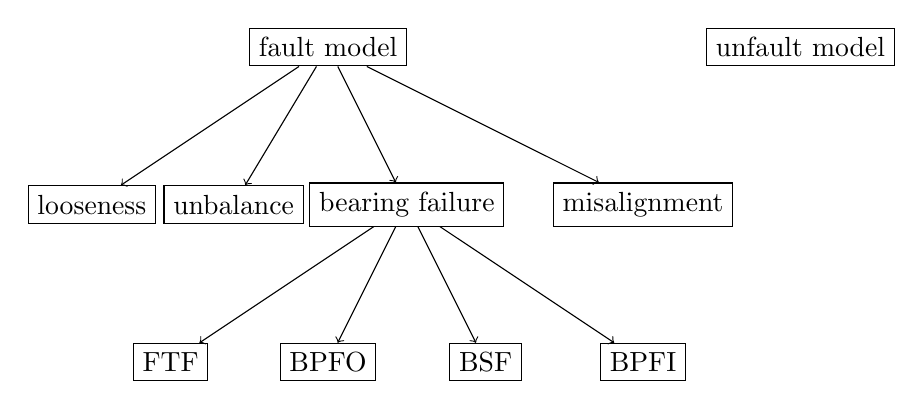
\begin{tikzpicture}
				\node (box1) [draw, rectangle] at (0,0) {unfault model};
				\node (box2) [draw, rectangle, left of=box1, node distance=6cm] {fault model};
				\node (box3) [draw, rectangle] at (-7.2,-2) {unbalance};
				\node (box4) [draw, rectangle] at (-2,-2) {misalignment};
				\node (box5) [draw, rectangle] at (-5,-2) {bearing failure};
				\node (box6) [draw, rectangle] at (-9,-2) {looseness};
				\node (box7) [draw, rectangle] at (-6,-4) {BPFO};
				\node (box8) [draw, rectangle] at (-2,-4) {BPFI};
				\node (box9) [draw, rectangle] at (-4,-4) {BSF};
				\node (box10) [draw, rectangle] at (-8,-4) {FTF};
				
				% Arrows
				\draw[->] (box2) -- (box3);
				\draw[->] (box2) -- (box4);
				\draw[->] (box2) -- (box5);
				\draw[->] (box2) -- (box6);
				\draw[->] (box5) -- (box7);
				\draw[->] (box5) -- (box8);
				\draw[->] (box5) -- (box9);
				\draw[->] (box5) -- (box10);
		\end{tikzpicture}}
		\caption{Unfault and fault model sub-categories} \label{fig:faultTree}
	\end{figure}
	\end{frame}
	
	
	\section{Challenges}

	\begin{frame}{Predictive Maintenance Challenges}
		Challenges in vibration analysis and predicting faulty components, with a focus on reinforcing reliability:
		\begin{itemize}
			\item Data Quality and Noise.		
			\item Complexity of Signal Processing.	
			\item Scalability and Real-Time Analysis.		
			\item Adaptability to Different Machinery.
			\item Reliability Metrics.
		\end{itemize}
	\end{frame}

	\section{Approaches}
	\subsection{Fault Type Classification}
	\begin{frame}{Fault Type Classification}
	\begin{figure}[h]
		\centering
		\resizebox{\columnwidth}{!}{
			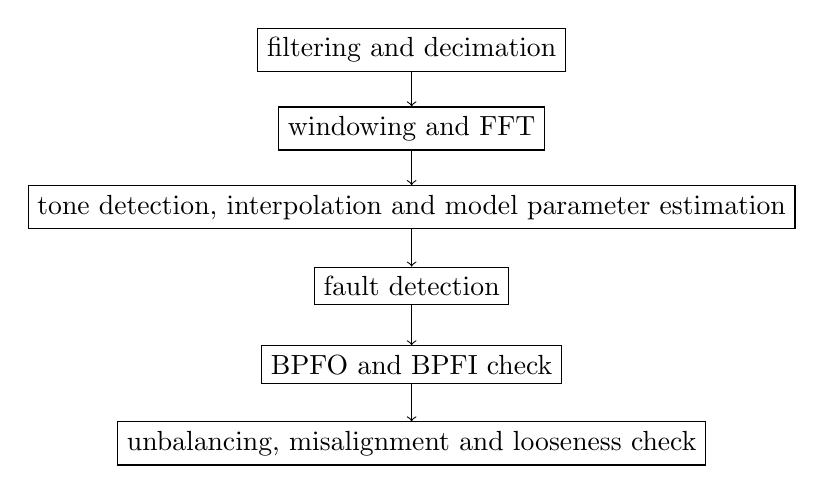
\begin{tikzpicture}
				\node (box1) [draw, rectangle] at (0,0) {filtering and decimation};
				\node (box2) [draw, rectangle, below of=box1, node distance=1cm] {windowing and FFT};
				\node (box3) [draw, rectangle, below of=box2, node distance=1cm] {tone detection, interpolation and model parameter estimation};
				\node (box4) [draw, rectangle, below of=box3, node distance=1cm] {fault detection};
				\node (box5) [draw, rectangle, below of=box4, node distance=1cm] {BPFO and BPFI check};
				\node (box6) [draw, rectangle, below of=box5, node distance=1cm] {unbalancing, misalignment and looseness check};
				
				% Arrows
				\draw[->] (box1) -- (box2);
				\draw[->] (box2) -- (box3);
				\draw[->] (box3) -- (box4);
				\draw[->] (box4) -- (box5);
				\draw[->] (box5) -- (box6);
			\end{tikzpicture}
		}
		\caption{The series of checks carried out by the algorithm}
		\label{fig:checks}
	\end{figure}	
	\end{frame}
	
	\subsection{Power Spectrum Density calculation}
	\begin{frame}{Power Spectrum Density calculation}
	Power Spectrum Density Threshold Calculation:
	
	\[
	\text{PSD} = \frac{(\text{Power Spectrum})^2}{\Delta f \times \text{Noise Power Bandwidth of Window}}
	\]
	Where: 
	\begin{itemize}
		\item Power spectrum is calculated by taking the average of the magnitude squared of multiple frequency spectra \[ PS = \frac{2 \times \text{X}^2}{N^2} \]
		\item \[ \Delta f  = \frac{f_{s}}{N} \] is the frequency resolution 
		\item Noise Power Bandwidth of Window is a correction factor for the rectangular window
	\end{itemize}
	\end{frame}
	
	\begin{frame}{Power Spectrum Density calculation}
	\begin{figure}[h]
		\centering
		\includegraphics[width=0.3\linewidth]{images/PSDCombinedloaded.png}
		\caption{Combination of all the aforementioned faults (inner case, outer case and bearing ball fault) \cite{Azeem2019}.}
		\label{fig:PSDCombinedloaded}
	\end{figure}
	\end{frame}
	
	\subsection{Dynamic signal stability analysis}
	\begin{frame}{Dynamic signal stability analysis}
	\begin{figure}[h]
		\centering
		\resizebox{\columnwidth}{!}{
			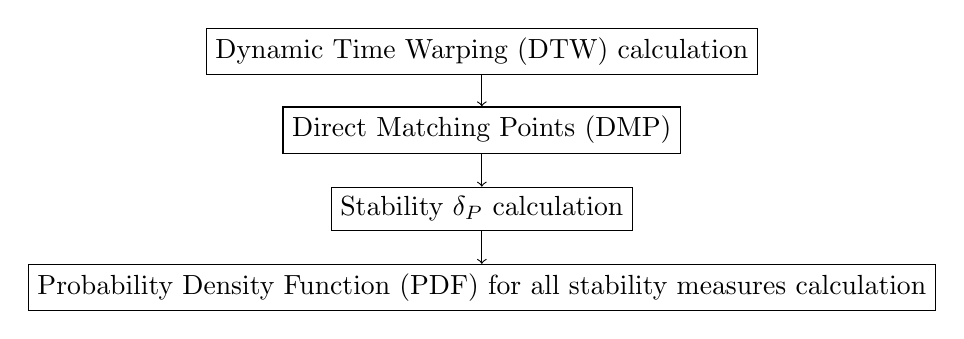
\begin{tikzpicture}
				\node (box1) [draw, rectangle] at (0,0) {Dynamic Time Warping (DTW) calculation};
				\node (box2) [draw, rectangle, below of=box1, node distance=1cm] {Direct Matching Points (DMP)};
				\node (box3) [draw, rectangle, below of=box2, node distance=1cm] {Stability $\delta_P$ calculation};
				\node (box4) [draw, rectangle, below of=box3, node distance=1cm] {Probability Density Function (PDF) for all stability measures calculation};
				
				
				% Arrows
				\draw[->] (box1) -- (box2);
				\draw[->] (box2) -- (box3);
				\draw[->] (box3) -- (box4);
				
			\end{tikzpicture}
		}
		\caption{The series of checks carried out by the algorithm}
		\label{fig:stabilityprocessflowdiagram}
	\end{figure}
	\end{frame}
	
	\subsection{Vibration Spectrum and phase analysis}
	\begin{frame}{ Vibration Spectrum and phase analysis}
	\begin{figure}[h]
		\centering
		\resizebox{\columnwidth}{!}{
			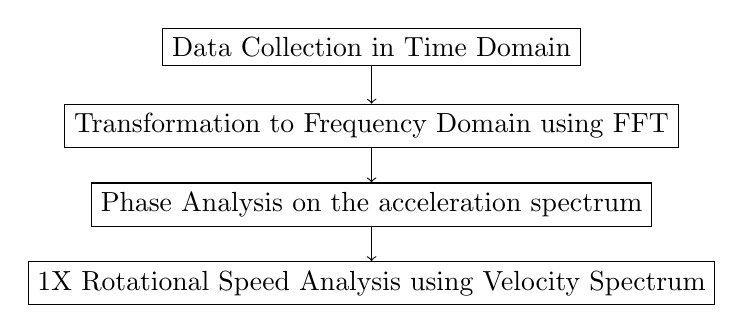
\begin{tikzpicture}
				\node (box1) [draw, rectangle] at (0,0) {Data Collection in Time Domain};
				\node (box2) [draw, rectangle, below of=box1, node distance=1cm] {Transformation to Frequency Domain using FFT};
				\node (box3) [draw, rectangle, below of=box2, node distance=1cm] {Phase Analysis on the acceleration spectrum};
				\node (box4) [draw, rectangle, below of=box3, node distance=1cm] {1X Rotational Speed Analysis using Velocity Spectrum};
				
				
				% Arrows
				\draw[->] (box1) -- (box2);
				\draw[->] (box2) -- (box3);
				\draw[->] (box3) -- (box4);
				
			\end{tikzpicture}
		}
		\caption{The series of checks carried out by the algorithm}
		\label{fig:specandphase}
	\end{figure}
	\end{frame}
	
	
	
	
	
	\subsection{Incipient SVM on time-domain}
		\begin{frame}{Incipient SVM Fault Detection Model and Anomaly Detection Model on time-domain dataset}	
		\begin{figure}[h]
			\centering
			\resizebox{\columnwidth}{!}{
				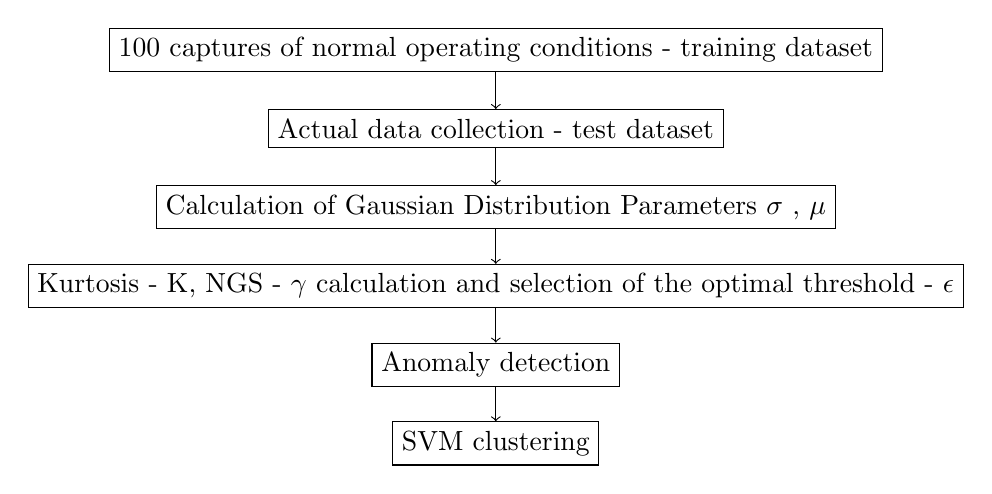
\begin{tikzpicture}
					\node (box1) [draw, rectangle] at (0,0) {100 captures of normal operating conditions - training dataset};
					\node (box2) [draw, rectangle, below of=box1, node distance=1cm] {Actual data collection - test dataset};
					\node (box3) [draw, rectangle, below of=box2, node distance=1cm] {Calculation of Gaussian Distribution Parameters $\sigma$ , $\mu$};
					\node (box4) [draw, rectangle, below of=box3, node distance=1cm] {Kurtosis - K, NGS - $\gamma$ calculation and selection of the optimal threshold - $\epsilon$};
					\node (box5) [draw, rectangle, below of=box4, node distance=1cm] {Anomaly detection};
					\node (box6) [draw, rectangle, below of=box5, node distance=1cm] {SVM clustering};
					
					% Arrows
					\draw[->] (box1) -- (box2);
					\draw[->] (box2) -- (box3);
					\draw[->] (box3) -- (box4);
					\draw[->] (box4) -- (box5);
					\draw[->] (box5) -- (box6);
				\end{tikzpicture}
			}
			\caption{Incipient SVM Model}
			\label{fig:svm}
		\end{figure}	
	\end{frame}


	\subsection{Incipient fault detection with one-class v-SVM algorithm}
	\begin{frame}{Incipient fault detection with one-class v-SVM algorithm}	
	\begin{figure}[h]
		\centering
		\resizebox{\columnwidth}{!}{
			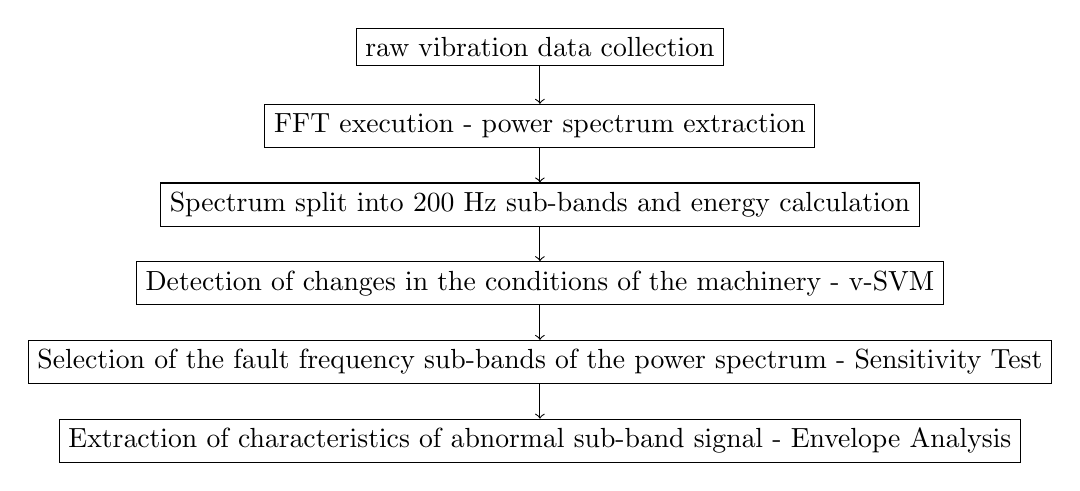
\begin{tikzpicture}
				\node (box1) [draw, rectangle] at (0,0) {raw vibration data collection};
				\node (box2) [draw, rectangle, below of=box1, node distance=1cm] {FFT execution - power spectrum extraction};
				\node (box3) [draw, rectangle, below of=box2, node distance=1cm] {Spectrum split into 200 Hz sub-bands and energy calculation};
				\node (box4) [draw, rectangle, below of=box3, node distance=1cm] {Detection of changes in the conditions of the machinery - v-SVM};
				\node (box5) [draw, rectangle, below of=box4, node distance=1cm] {Selection of the fault frequency sub-bands of the power spectrum - Sensitivity Test};
				\node (box6) [draw, rectangle, below of=box5, node distance=1cm] {Extraction of characteristics of abnormal sub-band signal - Envelope Analysis};
				
				% Arrows
				\draw[->] (box1) -- (box2);
				\draw[->] (box2) -- (box3);
				\draw[->] (box3) -- (box4);
				\draw[->] (box4) -- (box5);
				\draw[->] (box5) -- (box6);
			\end{tikzpicture}
		}
		\caption{Architecture of anomaly detection frequency sub-band \cite{Francos2013}}
		\label{fig:v-svm}
	\end{figure}
	\end{frame}
	
	
	\subsection{Real-time fault detection set-up with SVM algorithm}
	\begin{frame}{Real-time fault detection set-up with SVM algorithm}	
	\begin{figure}[h]
		\centering
		\resizebox{\columnwidth}{!}{
			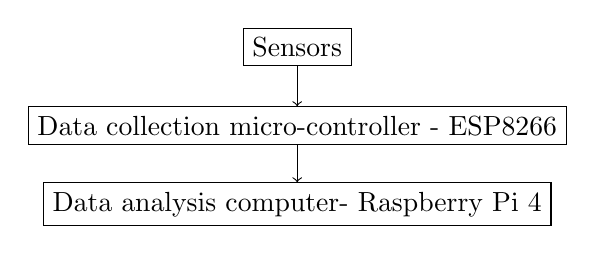
\begin{tikzpicture}
				\node (box1) [draw, rectangle] at (0,0) {Sensors};
				\node (box2) [draw, rectangle, below of=box1, node distance=1cm] {Data collection micro-controller - ESP8266};
				\node (box3) [draw, rectangle, below of=box2, node distance=1cm] {Data analysis computer- Raspberry Pi 4}; 
				
				% Arrows
				\draw[->] (box1) -- (box2);
				\draw[->] (box2) -- (box3);
				
			\end{tikzpicture}
		}
		\caption{Architecture of anomaly detection frequency sub-band \cite{Raman2023}}
		\label{fig:sensors}
	\end{figure}
	\end{frame}
	
	
	
	\subsection{Backpropagation Neural Network}
	\begin{frame}{Backpropagation Neural Network}	
	\begin{figure}[h]
		\centering
		\resizebox{\columnwidth}{!}{
			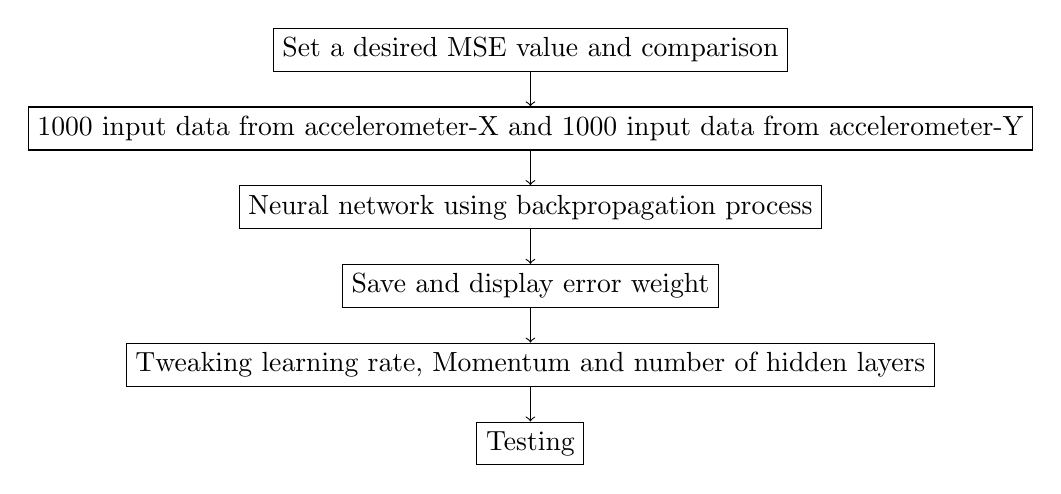
\begin{tikzpicture}
				\node (box1) [draw, rectangle] at (0,0) {Set a desired MSE value and comparison};
				\node (box2) [draw, rectangle, below of=box1, node distance=1cm] {1000 input data from accelerometer-X and 1000 input data from accelerometer-Y};
				\node (box3) [draw, rectangle, below of=box2, node distance=1cm] {Neural network using backpropagation process}; 
				\node (box4) [draw, rectangle, below of=box3, node distance=1cm] {Save and display error weight};
				\node (box5) [draw, rectangle, below of=box4, node distance=1cm] {Tweaking learning rate, Momentum and number of hidden layers};
				\node (box6) [draw, rectangle, below of=box5, node distance=1cm] {Testing};
				
				% Arrows
				\draw[->] (box1) -- (box2);
				\draw[->] (box2) -- (box3);
				\draw[->] (box3) -- (box4);
				\draw[->] (box4) -- (box5);
				\draw[->] (box5) -- (box6);
			\end{tikzpicture}
		}
		\caption{Flowchart for the Backpropagation-Neural Network (B-NN) training and testing \cite{Kuspijani2020}.}
		\label{fig:BNNflowchart}
	\end{figure}
	\end{frame}
	
	
	
	
	

	\section{Conclusions}
	\begin{frame}
		\begin{itemize}
			\item \textbf{Vibration Analysis Techniques:} Wide variety including time-domain and frequency-domain analysis.
			
			\item \textbf{Fault Detection Algorithms:} Use parameters or thresholds for classification, highly effective for assessing machinery health. Dynamic signal stability analysis is a standout tool.
			
			\item \textbf{Machine Learning Anomaly Detection:} Can be combined with root algorithms, focus on continuous monitoring and past data analysis in specific application contexts.
		\end{itemize}
	\end{frame}
	
	
	
	
	
	
%	
%	
%	
%	\section{References}
%	
%	\begin{frame}[allowframebreaks]
%		\renewcommand{\refname}{References} 
%		\bibliographystyle{ieeetr}
%		\bibliography{references}
%		\nocite{*} % used here because no citation happens in slides
%		% if there are too many try use:
%		% \tiny\bibliographystyle{alpha}
%	\end{frame}
%	
%	
%	\begin{frame}
%		\begin{center}
%			{\Huge\calligra Thank You}
%		\end{center}
%	\end{frame}
	
\end{document}